\section{Hardware Design Sensorknoten}
\label{sec:HardwareDesign}
In diesem Unterkapitel wird das Design des Sensorknotens, sowie der Produktionsprozess näher betrachtet. Es wird dabei zuerst auf den energiesparenden Sensorknoten, der mit dem Arduino Pro Mini realisiert wurde, und anschließend auf den normalen Sensorknoten, der mit dem Arduino Nano eingegangen.
\subsection{Arduino Pro Mini}
\begin{figure}
	\centering
	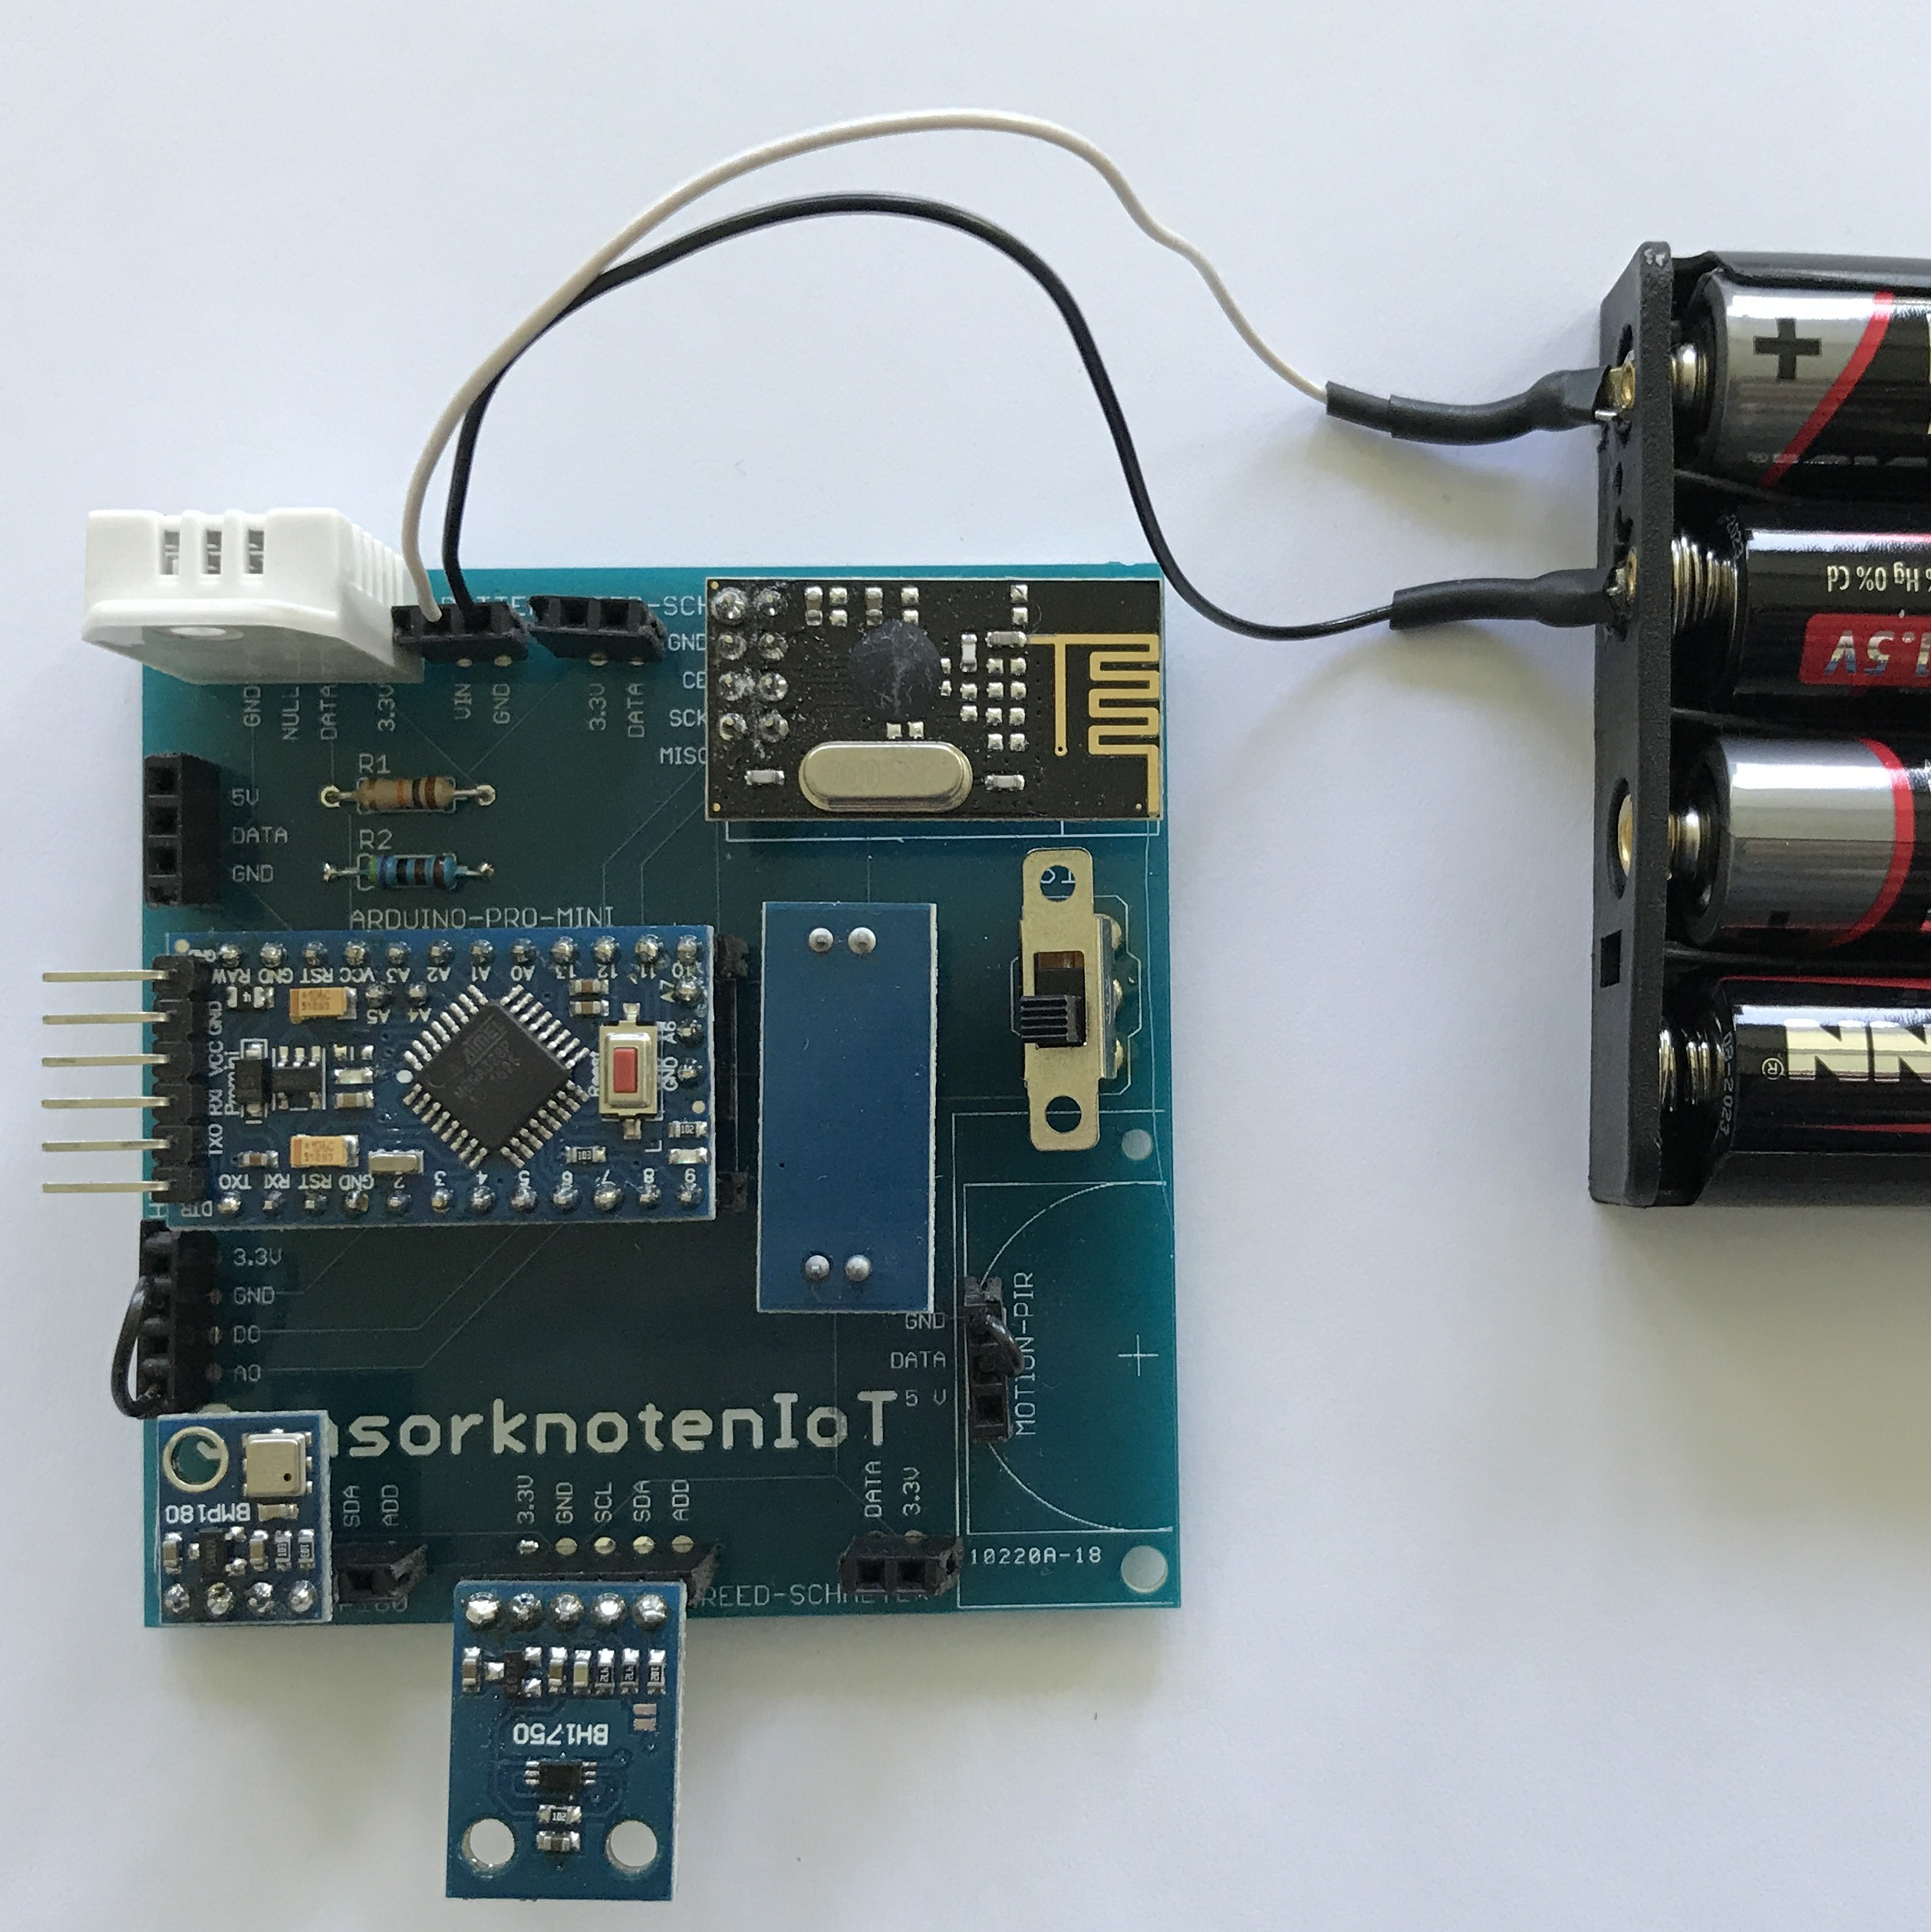
\includegraphics[width=0.6\textwidth]{bilder/mini_cutted}
	\caption[Energiesparender Sensorknoten]{Energiesparender Sensorknoten: bestückt mit verschiedenen Sensoren und einem Arduino Pro Mini}
	\label{img:ArduinoProMini}
\end{figure}
Der energiesparende Sensorknoten wird dauerhaft mit Batterien betrieben, dieser ist in Bild \ref{img:ArduinoProMini} zu sehen. Der Sensorknoten ist mit einem Arduino Pro Mini bestückt, da dieser energiesparender ist als der Arduino Nano. Bei Sensorknoten lassen sich mit den in Kapitel \ref{sec:VerwendeteSensoren} vorgestellten Sensoren bestücken. Die Sensoren können mit Hilfe von Stiftleisten jederzeit getauscht werden, nur beim DHT22 bzw. DHT11 haben wir uns entschieden diesen direkt aufzulöten. Der Grundgedanke war dabei, dass jeder Sensorknoten als Mindestanforderung die Temperatur und Luftfeuchtigkeit bestimmen kann. Jeder Sensorknoten besitzt ein nRF24L01 Modul zur Kommunikation mit anderen Sensorknoten oder dem Raspberry Pi.
\paragraph{Spannungsversorgung} Der Arduino Pro Mini verfügt über kein 5V zu 3,3V Wandler, weshalb zusätzlich noch ein Wandler aufgebracht wurde. Dieser 5V zu 3,3V Wandler ist ebenfalls nur mit Hilfe von Stiftleisten aufgebracht. 

Die Spannungsversorgung des Sensorknoten erfolgt mit 4 x 1,5 AA Batterien, diese liefern gemeinsam eine Spannung von 6V zu Beginn ihrer Betriebszeit. Der Sensorknoten kann bis ca. 4,2V betrieben werden. Die Spannungszufuhr kann mit Hilfe eines Schalters unterbrochen werden. 
\paragraph{Aufgetretene Probleme} Bei der Erstellung des Schaltplans ist ein Fehler bei Sensorschnittstellen für den BMP180 und BH1750 entstanden. Beide Sensoren werden über das $I^2C$ Schnittstelle angesprochen. Hierbei kam es zu einer Vertauschung der 3,3V Leitung und der Masse Leitung. Aus diesem Grund können diese beiden Sensoren nur mit einem Adapter bzw. mit flexiblen Steckbrücken betrieben werden. Die Funktion der Schnittstelle sind davon nicht betroffen. 

Zusätzlich kam es bei der Auswertung der Reed-Kontakte zu zufälligen falschen Werten. Diese konnte behoben werden in dem ein zusätzlicher 10k Ohm Pull Down-Widerstand eingelötet wurde, der das Signal auf Masse zieht.

Um zusätzlich zufällige Werte auszuschließen, wenn kein Bewegungsmelder oder Bodenfeuchtigkeitsmesser angeschlossen ist, wurde eine Steckbrücke genutzt. Diese Steckbrücke verbindet die Datenleitung mit Masse.  Durch dieses Verfahren kann einfach überprüft werden ob die Sensoren angeschlossen sind oder nicht.
\label{sec:ArduinoProMini}
\subsection{Arduino Nano}
\label{sec:ArduinoNano}
\begin{figure}
	\centering
	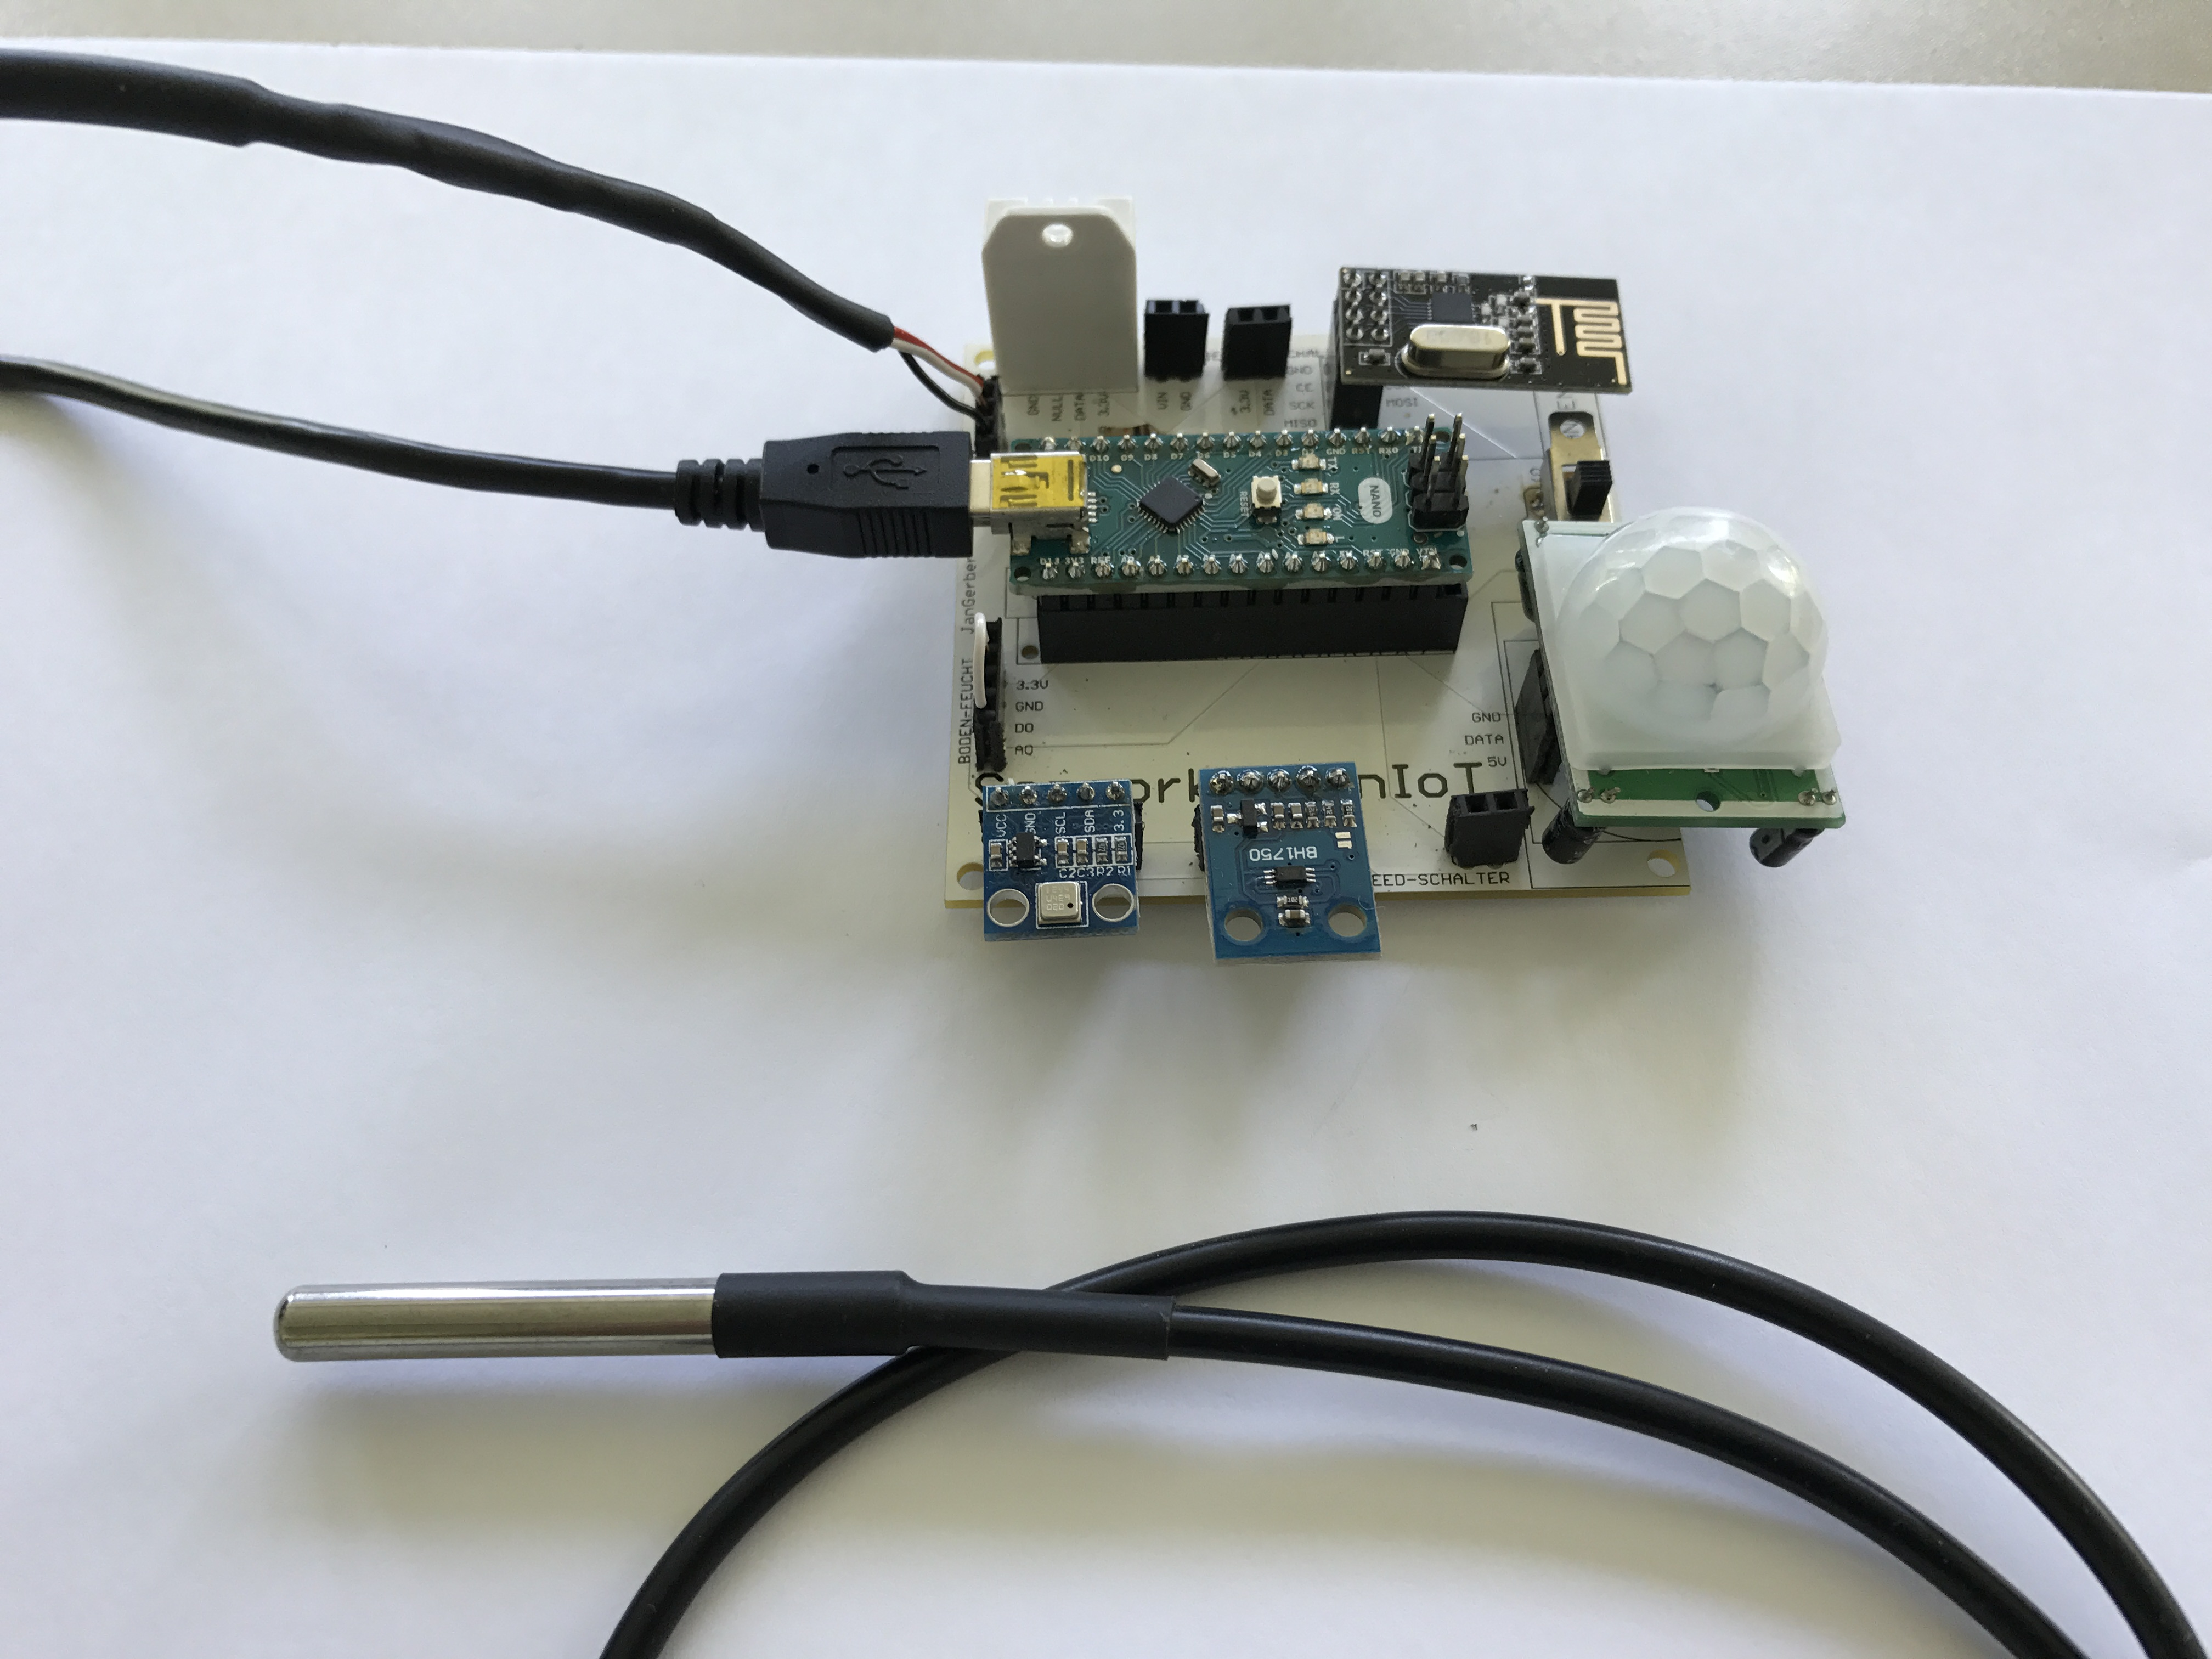
\includegraphics[width=0.6\textwidth]{bilder/SensorknotenArduinoNano}
	\caption[Normaler Sensorknoten]{Normaler Sensorknoten: bestückt mit verschiedenen Sensoren und einem Arduino Nano}
	\label{img:ArduinoNano}
\end{figure}
Der normale Sensorknoten ist mit einem Arduino Nano bestückt. Dieser verfügt über die gleichen Anschlussmöglichkeiten wie der energiesparende Sensorknoten. In Bild \ref{img:ArduinoNano} ist der normale Sensorknoten zu sehen.
\paragraph{Spannungsversorgung} Der normale Sensorknoten kann entweder über die vorhandene USB Schnittstelle betrieben werden oder ebenfalls wie der Arduino Pro Mini über eine externe Stromversorgung, wie zum Beispiel Batterien oder Akkus. Da diese Sensorknoten jedoch deutlich mehr Energie benötigt als der energiesparende Sensorknoten, sollten genügend mAh zur Verfügung stellen. Die externe Stromversorgung kann über ein Schalter ausgeschalten werden. Der Arduino Nano verfügt direkt auf dem Board ein Wandler von 5V zu 3,3V.
\paragraph{Aufgetretene Probleme} Mit dem normalen Board sind die gleichen Probleme hinsichtlich dem Einsatz von Widerständen aufgetreten, diese Probleme konnten wie beim energiesparende Sensorknoten gelöst werden. Das Sensorknoten Board war allerdings vollständig richtig, was das aufbringen und wechseln von Sensoren deutlich erleichtert.
\subsection{Produktionsprozess der Sensorknoten}
\label{sec:ProduktionsprozessSensornoten}
In diesem Unterkapitel wird auf den gesamten Produktionsprozess eingegangen. Beginnend mit der Entwicklung eines Prototypens, über die Erstellung genauer Schaltpläne und abschließend mit der Bestellung der Platinen, sowie der Bestückung dieser Platinen.
\paragraph{Erstellung eines Prototypen} Um sich in das Thema einzuarbeiten, wurde zunächst ein Prototyp entwickelt ( siehe Bild \ref{img:prototyp}. Dieser wurde auf einer einfachen Lochrasterplatine entwickelt. Die einzelnen Komponenten wurden mit Drahtstücken verbunden. Der Löt- und Bestückungsvorgang ging pro Prototyp 2-3 Stunden. Auf dem Prototyp war das Funkmodul, der DHT22 Sensor und eine Sensor mit einer $I^2C$ Schnittstelle aufgebracht. Alle Sensoren konnten in Steckleisten befestigt werden, dies ermöglichte einen schnellen Austausch falls ein Sensor ausfallen würde. Für die Erstellung der Prototypen wurde ein handschriftlicher Schaltplan entworfen.
\begin{figure}
	\centering
	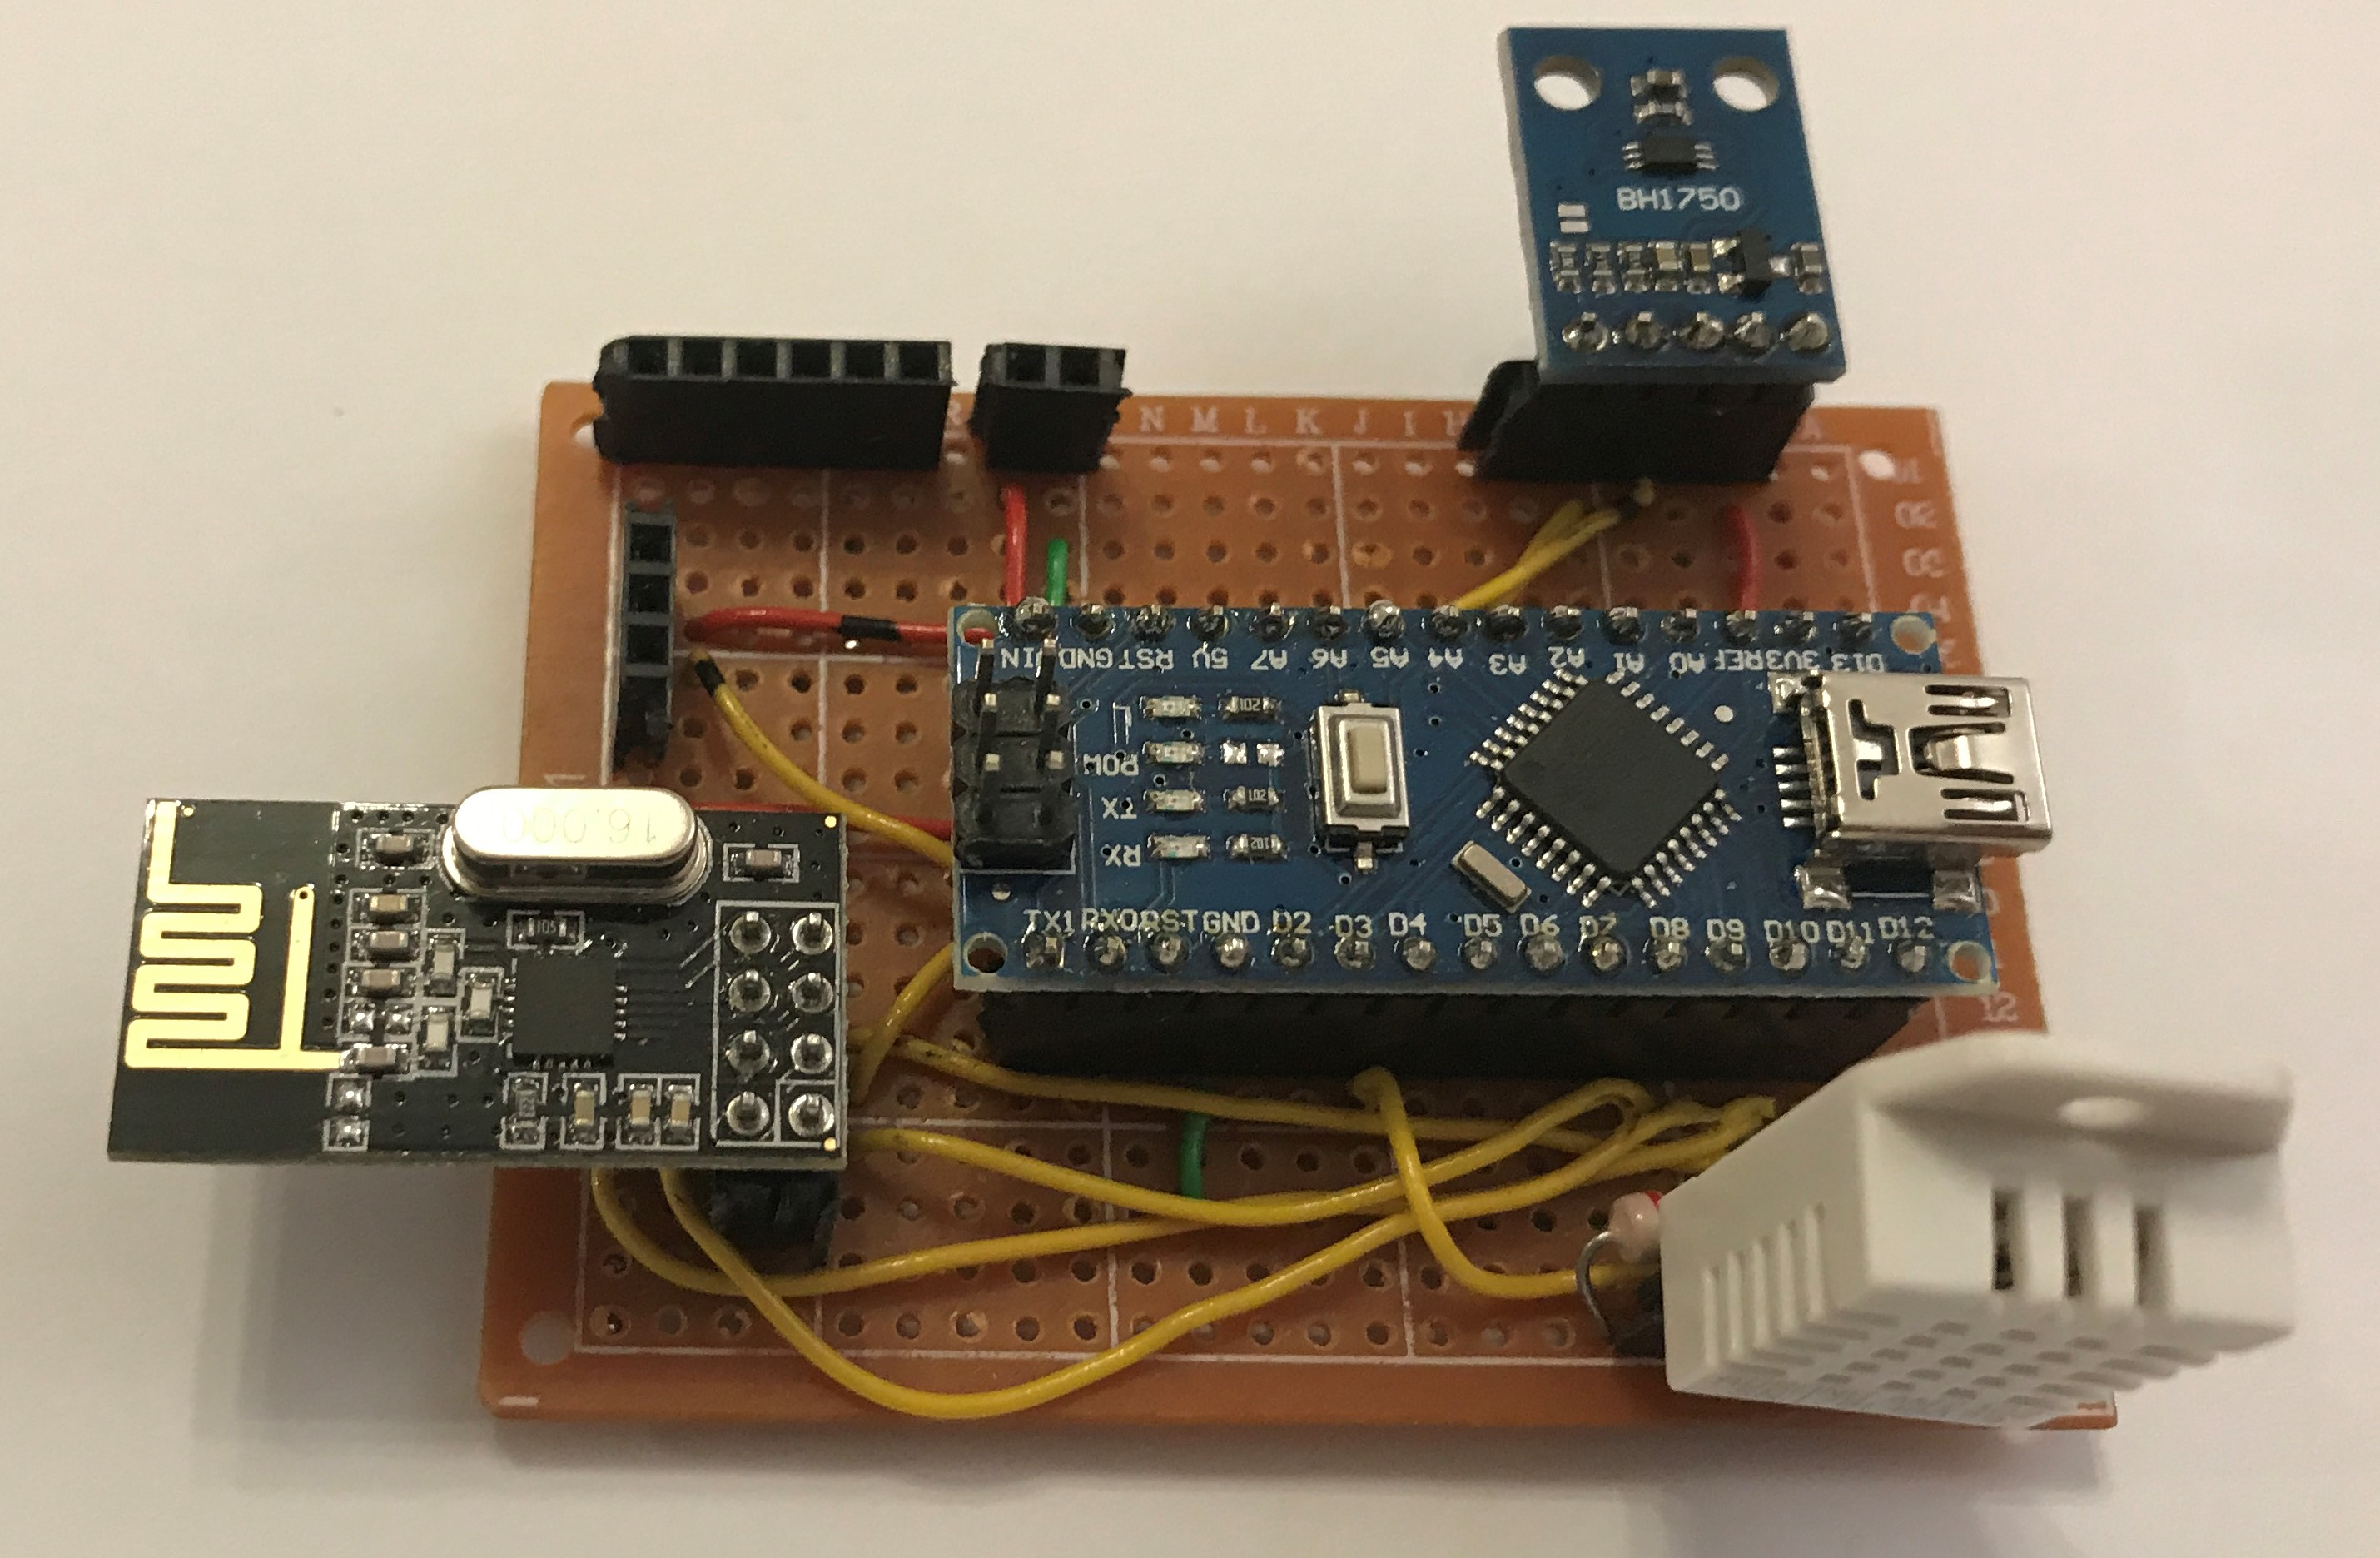
\includegraphics[width=0.6\textwidth]{bilder/prototyp}
	\caption[Prototyp Sensorknoten]{ Prototyp Sensorknoten bestückt mit einem Arduino Nano, DHT22 und dem nRF24l01 Funkmodul und wahlweise mit einem BH1750 oder BMP180}
	\label{img:prototyp}
\end{figure}

\paragraph{Erstellung eines Schaltplans} Nachdem ein funktionsfähiger Prototyp entworfen wurde, konnte ein Schaltplan für den energiesparenden Sensorknoten und den normalen Sensorknoten entwickelt werden. Die Schaltpläne beider Sensorknoten sind im Anhang zu finden. Der Schaltplan wurde komplett entworfen ohne alle Bauteile getestet zu haben. Zusätzlich wurde nur für den normalen Sensorknoten ein Prototypen entworfen, da zum Zeitpunkt der Erstellung des Prototyen die Arduino Pro Mini nicht vorlagen. Der Schaltplan wurde mit Hilfe von Eagle (siehe Kapitel \ref{sec:MesswerterfassungArduino} erstellt.
\paragraph{Erstellung eines Layouts} Eagle bietet die Möglichkeit, nach der Erstellung eines Schaltplans ein Layout für diesen Schaltplan zu entwickeln. Zunächst muss die Größe der Platine festgelegt werden, diese ist bei den Sensorknoten 70 mm * 69 mm. Im nächsten Schritt werden alle Bauteile auf der Platine platziert und positioniert. Nachdem die Bauteile so positioniert worden sind, dass genügend Platz zwischen den Bauteilen ist. Können die Leiterbahnen Routen, mit Hilfe des Autorouters auf der Leiterplatte verlegt werden. Die Leiterbahnen werden nach bereits vorher angegeben Anforderungen (zum Beispiel Abstand und Breite Leiterbahnen) verlegt. Im letzten Schritt wird die Platine noch beschriftet und Bohrlöcher in den Ecken hinzugefügt. So besteht auch die Möglichkeit die Platinen in einem Gehäuse zu befestigen. 
\paragraph{Bestellprozess} Da das Erstellen der Platinen Zeitaufwendig wäre haben wir uns entschieden die Platinen produzieren zu lassen. Nach einem kurzen Vergleich verschiedener Hersteller, 
\paragraph{Bestückung de Platinen}
